\begin{table*}[!t]
    \centering
    \footnotesize
    \begin{minipage}[t]{0.56\textwidth}
        \centering
    \caption{Ablation results on ScreenSpot-v2 and ScreenSpot-Pro of coordinate-free GUI grounding methods fine-tuned with a 45k ablation dataset. Variants in \colorbox{blue!10}{blue} represent the selected settings for \method{}.}
    % \vspace{-0.5em}
    \resizebox{\linewidth}{!}{
    % \begin{tabular}{y{160}cccccc}
    \begin{tabular}{p{160pt}cccccc}
        \toprule
        \multirow{2}{*}{\textbf{Model}} & \multicolumn{3}{c@{\hspace{1em}}}{\textbf{ScreenSpot-v2}$\uparrow$} & \multicolumn{3}{c@{\hspace{1em}}}{\textbf{ScreenSpot-Pro}$\uparrow$}\\
        & Text & Icon & \textbf{Avg.}& Text & Icon & \textbf{Avg.} \\
        \midrule
        \rowcolor{gray!30} 
        \multicolumn{7}{l}{\textit{Existing Coordinate-free GUI Grounding}} \\
        GUI-Actor-3B (45k) & 96.24 & 75.99 & 87.42 & 50.67 & 12.25 & 35.99 \\
        Vanilla Attention Grounding (45k) & 95.68 & 75.45 & 86.87 & 53.02 & 12.42 & 37.51 \\
        \midrule
        \rowcolor{gray!30} 
        \multicolumn{7}{l}{\textit{Simplified Attention Grounding: GUI-AIMA-3B (45k)}} \\
        \rowcolor{gray!10}\multicolumn{7}{l}{\textit{Attention Head Weighting without $\mathcal{Q}_s$} in \cref{eq:unified_head_score}}\\
        + weighting uniformly & 97.08 & 78.34 & 88.92 & 56.50 & 13.91 & 40.23 \\
        + weighting with all $\mathcal{Q}'=\mathcal{Q}$ & 96.24 & 78.34 & 88.44 & 52.61 & 13.41 & 37.63 \\
        + weighting with $\mathcal{Q}'=\{\texttt{<ANCHOR>}\}$ & 96.66 & 76.35 & 87.81 & 56.91 & 14.57 & 40.73 \\
        \rowcolor{gray!10}\multicolumn{7}{l}{\textit{Attention Head Weighting with }$\mathcal{Q}'=\mathcal{Q}_s$\textit{ in} \cref{eq:unified_head_score}}\\
        + layer-wise $\operatorname{top-1} \mathcal{Q}_s^l$ & 96.52 & \textbf{81.23} & \textbf{89.86} & 57.32 & \underline{15.73} & 41.43 \\
        + layer-wise $\operatorname{top-3} \mathcal{Q}_s^l$ & 96.66 & 79.06 & 88.99 & 57.83 & \underline{15.07} & 41.49 \\
        \rowcolor{blue!10}
        + global $\operatorname{top-1} \mathcal{Q}_s$ & \textbf{97.49} & 78.88 & 89.39 & \underline{59.26} & 14.40 & \underline{42.13} \\
        + global $\operatorname{top-3} \mathcal{Q}_s$ & 95.82 & 70.94 & 84.98 & 57.01 & 14.40 & 40.73 \\
        \rowcolor{blue!10}
        ~~~~ + weighted patch-wise labeling & \underline{97.21} & \underline{79.60} & \underline{89.54} & \textbf{61.00} & 14.90 & \textbf{43.39} \\
        \bottomrule
      \end{tabular}}
    % \vspace{-2em}
    \label{tab:ablation}
\end{minipage}
    \hfill
    \begin{minipage}[t]{0.4\textwidth}
    \captionsetup{type=figure}
    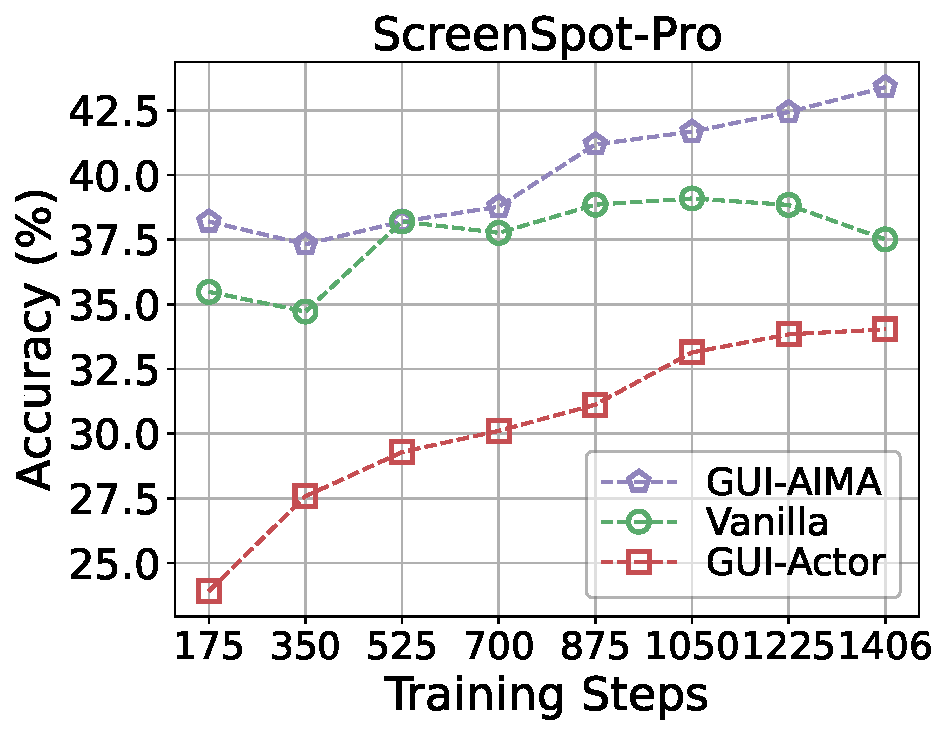
\includegraphics[width=\linewidth]{fig/convergence_ablation.pdf}
    \vspace{-2em}
    \caption{Model convergence of the 45k ablation dataset on ScreenSpot-Pro benchmark. %of \method{}, GUI-Actor and vanilla attention grounding.
    }
    \label{fig:Convergence}
    \end{minipage}
\end{table*}